\begin{figure}[h!]
	\centering
	
	
	
	\tikzset{every picture/.style={line width=0.75pt}} %set default line width to 0.75pt        
	
	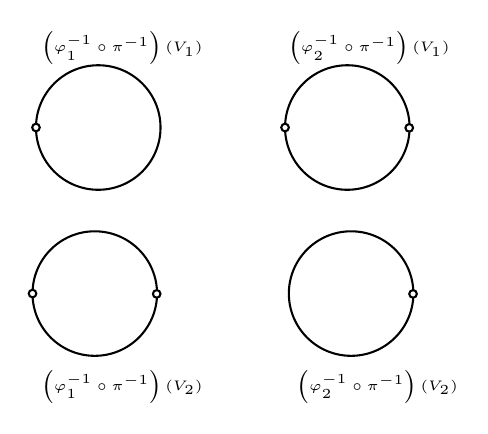
\begin{tikzpicture}[x=0.75pt,y=0.75pt,yscale=-1,xscale=1]
		%uncomment if require: \path (0,300); %set diagram left start at 0, and has height of 300
		
		%Shape: Circle [id:dp7624927902795768] 
		\draw   (90,80) .. controls (90,63.43) and (103.43,50) .. (120,50) .. controls (136.57,50) and (150,63.43) .. (150,80) .. controls (150,96.57) and (136.57,110) .. (120,110) .. controls (103.43,110) and (90,96.57) .. (90,80) -- cycle ;
		%Shape: Circle [id:dp8279394743167126] 
		\draw  [fill={rgb, 255:red, 255; green, 255; blue, 255 }  ,fill opacity=1 ] (88.17,80) .. controls (88.17,78.99) and (88.99,78.17) .. (90,78.17) .. controls (91.01,78.17) and (91.83,78.99) .. (91.83,80) .. controls (91.83,81.01) and (91.01,81.83) .. (90,81.83) .. controls (88.99,81.83) and (88.17,81.01) .. (88.17,80) -- cycle ;
		%Shape: Circle [id:dp9009991128602786] 
		\draw   (210,80) .. controls (210,63.43) and (223.43,50) .. (240,50) .. controls (256.57,50) and (270,63.43) .. (270,80) .. controls (270,96.57) and (256.57,110) .. (240,110) .. controls (223.43,110) and (210,96.57) .. (210,80) -- cycle ;
		%Shape: Circle [id:dp06103467761022641] 
		\draw  [fill={rgb, 255:red, 255; green, 255; blue, 255 }  ,fill opacity=1 ] (208.17,80) .. controls (208.17,78.99) and (208.99,78.17) .. (210,78.17) .. controls (211.01,78.17) and (211.83,78.99) .. (211.83,80) .. controls (211.83,81.01) and (211.01,81.83) .. (210,81.83) .. controls (208.99,81.83) and (208.17,81.01) .. (208.17,80) -- cycle ;
		%Shape: Circle [id:dp10180676331611016] 
		\draw  [fill={rgb, 255:red, 255; green, 255; blue, 255 }  ,fill opacity=1 ] (268,80.17) .. controls (268,79.15) and (268.82,78.33) .. (269.83,78.33) .. controls (270.85,78.33) and (271.67,79.15) .. (271.67,80.17) .. controls (271.67,81.18) and (270.85,82) .. (269.83,82) .. controls (268.82,82) and (268,81.18) .. (268,80.17) -- cycle ;
		%Shape: Circle [id:dp855196723421777] 
		\draw   (88.33,160) .. controls (88.33,143.43) and (101.76,130) .. (118.33,130) .. controls (134.9,130) and (148.33,143.43) .. (148.33,160) .. controls (148.33,176.57) and (134.9,190) .. (118.33,190) .. controls (101.76,190) and (88.33,176.57) .. (88.33,160) -- cycle ;
		%Shape: Circle [id:dp4627947669837389] 
		\draw  [fill={rgb, 255:red, 255; green, 255; blue, 255 }  ,fill opacity=1 ] (86.5,160) .. controls (86.5,158.99) and (87.32,158.17) .. (88.33,158.17) .. controls (89.35,158.17) and (90.17,158.99) .. (90.17,160) .. controls (90.17,161.01) and (89.35,161.83) .. (88.33,161.83) .. controls (87.32,161.83) and (86.5,161.01) .. (86.5,160) -- cycle ;
		%Shape: Circle [id:dp14067791390529916] 
		\draw  [fill={rgb, 255:red, 255; green, 255; blue, 255 }  ,fill opacity=1 ] (146.33,160.17) .. controls (146.33,159.15) and (147.15,158.33) .. (148.17,158.33) .. controls (149.18,158.33) and (150,159.15) .. (150,160.17) .. controls (150,161.18) and (149.18,162) .. (148.17,162) .. controls (147.15,162) and (146.33,161.18) .. (146.33,160.17) -- cycle ;
		%Shape: Circle [id:dp4395956628276514] 
		\draw   (211.83,160) .. controls (211.83,143.43) and (225.26,130) .. (241.83,130) .. controls (258.4,130) and (271.83,143.43) .. (271.83,160) .. controls (271.83,176.57) and (258.4,190) .. (241.83,190) .. controls (225.26,190) and (211.83,176.57) .. (211.83,160) -- cycle ;
		%Shape: Circle [id:dp3289592382066828] 
		\draw  [fill={rgb, 255:red, 255; green, 255; blue, 255 }  ,fill opacity=1 ] (269.83,160.17) .. controls (269.83,159.15) and (270.65,158.33) .. (271.67,158.33) .. controls (272.68,158.33) and (273.5,159.15) .. (273.5,160.17) .. controls (273.5,161.18) and (272.68,162) .. (271.67,162) .. controls (270.65,162) and (269.83,161.18) .. (269.83,160.17) -- cycle ;
		
		% Text Node
		\draw (91,32.4) node [anchor=north west][inner sep=0.75pt]  [font=\tiny]  {$\left( \varphi _{1}^{-1} \circ \pi ^{-1}\right)( V_{1})$};
		% Text Node
		\draw (210,32.4) node [anchor=north west][inner sep=0.75pt]  [font=\tiny]  {$\left( \varphi _{2}^{-1} \circ \pi ^{-1}\right)( V_{1})$};
		% Text Node
		\draw (91,195.4) node [anchor=north west][inner sep=0.75pt]  [font=\tiny]  {$\left( \varphi _{1}^{-1} \circ \pi ^{-1}\right)( V_{2})$};
		% Text Node
		\draw (214,195.4) node [anchor=north west][inner sep=0.75pt]  [font=\tiny]  {$\left( \varphi _{2}^{-1} \circ \pi ^{-1}\right)( V_{2})$};
		
		
	\end{tikzpicture}
\end{figure}